\documentclass{article}

% NeurIPS 2024 style
\usepackage[final]{neurips_2024}

\usepackage[utf8]{inputenc}
\usepackage[T1]{fontenc}
\usepackage{hyperref}
\usepackage{url}
\usepackage{booktabs}
\usepackage{graphicx}
\usepackage{amsmath}
\usepackage{amssymb}
\usepackage{subcaption}
\usepackage{caption}
\usepackage{natbib}
\usepackage{microtype}
\usepackage{algorithm}
\usepackage{algorithmic}
\usepackage{xcolor}
\usepackage{colortbl}
\usepackage{multirow}
\usepackage{float}

\title{MedGuard: Uncertainty-Aware Hybrid Classification\\for Robust Medical Vision}

\author{
  Ritesh Patil (230056) \\
  Rishihood University \\
  \And
  Harshal Nerpagar (230076) \\
  Rishihood University \\
}

\begin{document}

\maketitle

% ============================================================
% ABSTRACT
% ============================================================
\begin{abstract}
Automated pathology image classification has the potential to reduce diagnostic workload and improve clinical consistency, yet deploying such systems safely demands more than high accuracy---it requires reliable uncertainty estimation. An overconfident misclassification can cascade into incorrect treatment, making it critical that a model can distinguish what it knows from what it does not. In this work we present \textbf{MedGuard}, a three-tier classification framework evaluated on PathMNIST, a nine-class colorectal cancer tissue benchmark containing 107,180 images. We first establish a classical baseline by extracting Histogram of Oriented Gradients (HOG) features and training an RBF-kernel Support Vector Machine, achieving 42.5\% macro F1. We then fine-tune a ResNet18 backbone with class-weighted cross-entropy loss, early stopping, and data augmentation, reaching 91.9\% macro F1---a \textbf{116.3\% relative improvement}. Finally, we introduce a hybrid uncertainty layer that fits a Gaussian Mixture Model (GMM) on the penultimate-layer embeddings of the trained ResNet, enabling out-of-distribution (OOD) detection via log-likelihood thresholding at the 5\textsuperscript{th} training-set percentile. The hybrid layer flags 25.2\% of test samples as OOD; on the remaining in-distribution subset, accuracy rises from 93.7\% to \textbf{97.3\%} and macro F1 from 91.9\% to \textbf{95.8\%}, representing a 57\% reduction in classification errors. MedGuard combines deep feature extraction with density-based uncertainty estimation to provide a principled mechanism for flagging unreliable predictions---a capability absent from standard classification pipelines.
\end{abstract}

% ============================================================
% 1. INTRODUCTION
% ============================================================
\section{Introduction}
\label{sec:intro}

A 2023 study by the Leapfrog Group found that diagnostic errors affect approximately 7.4 million patients annually in United States emergency departments alone, with AI-assisted pathology systems increasingly deployed to mitigate this burden. Yet standard deep learning classifiers output a softmax probability that is frequently miscalibrated: a model may assign 95\% confidence to a prediction that is categorically wrong~\citep{gal2016dropout}. In safety-critical domains such as medical imaging, this overconfidence is not merely a statistical nuisance---it is a direct patient safety hazard.

The core safety argument motivating this work is straightforward: \emph{a model that says ``I don't know'' is safer than one that says ``I'm 95\% sure'' when it is wrong.} Current medical image classifiers, including those trained on the MedMNIST benchmark~\citep{yang2023medmnist}, lack an explicit mechanism to reject out-of-distribution (OOD) inputs. When presented with an image from an unseen tissue type or an artefact-corrupted slide, these models still produce a confident class prediction with no warning to the clinician.

MedGuard addresses this gap through a three-tier pipeline (Figure~\ref{fig:architecture}). Our contributions are:
\begin{enumerate}
    \item A classical ML baseline (HOG~+~SVM) that provides interpretable feature-level insight into tissue classification, with analysis of precisely where handcrafted features fail on fine-grained pathology data.
    \item A fine-tuned ResNet18 with class-weighted loss, data augmentation, and early stopping, demonstrating a \textbf{116.3\% relative F1 improvement} over the baseline while documenting its overconfidence failure mode on OOD inputs.
    \item A hybrid uncertainty layer that fits a Gaussian Mixture Model on ResNet embeddings and uses log-likelihood thresholding for OOD detection, enabling the system to \emph{abstain} rather than misclassify---improving in-distribution accuracy to 97.3\% by filtering unreliable predictions.
\end{enumerate}

\begin{figure}[t]
\centering
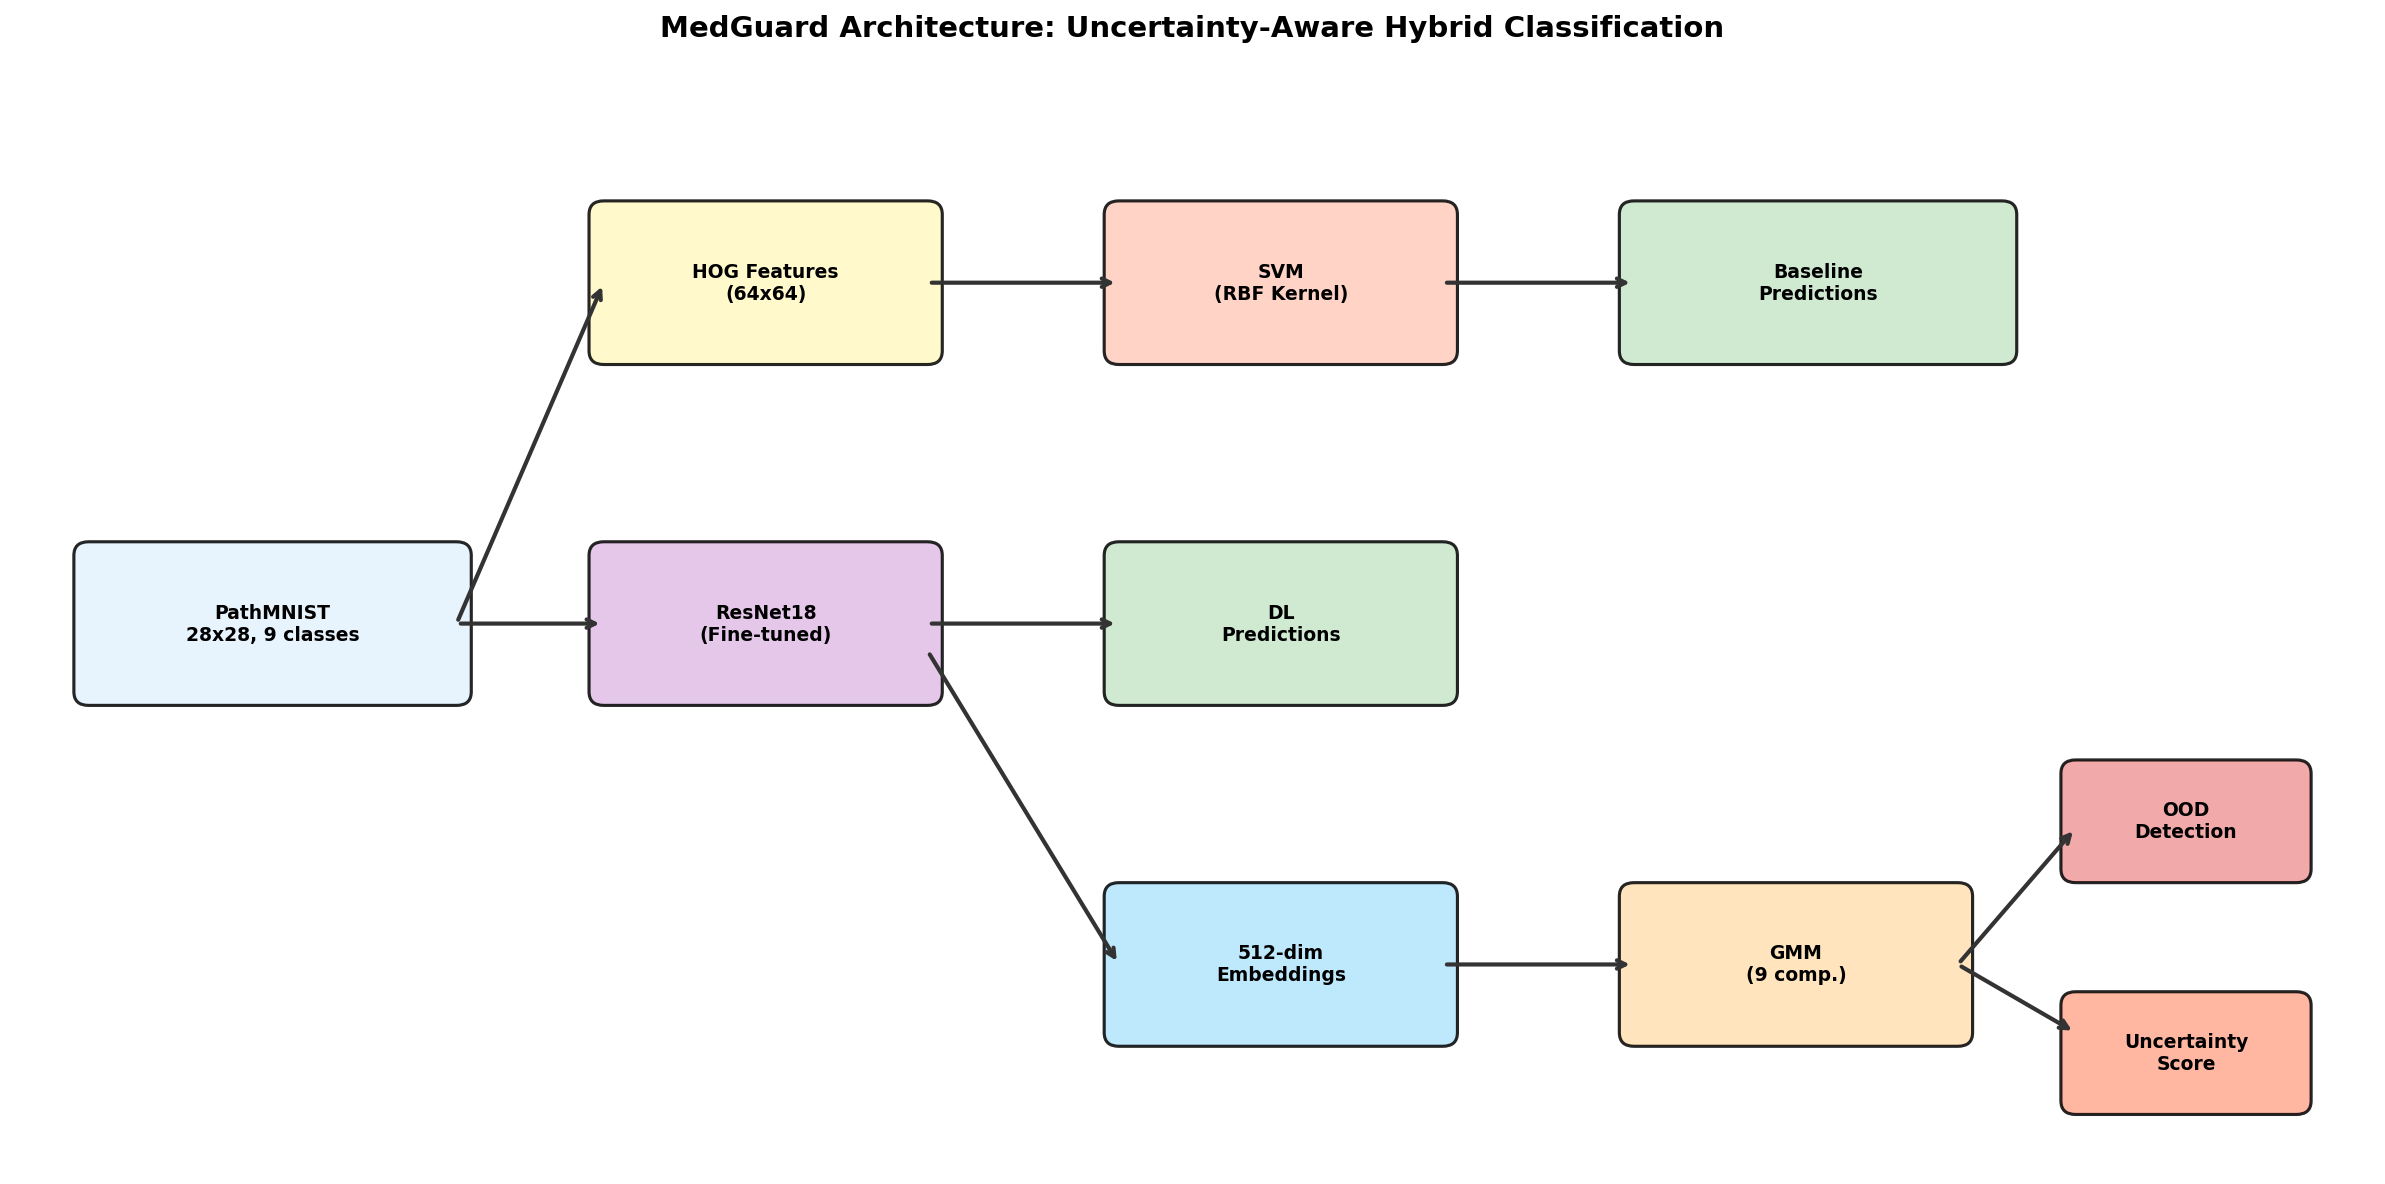
\includegraphics[width=0.95\textwidth]{figures/architecture_diagram.png}
\caption{MedGuard system architecture. The three-tier pipeline processes input images through a classical HOG+SVM baseline (Tier~1), a fine-tuned ResNet18 classifier (Tier~2), and a GMM-based uncertainty layer on ResNet embeddings (Tier~3). Tier~3 enables the system to abstain on out-of-distribution inputs rather than producing overconfident misclassifications.}
\label{fig:architecture}
\end{figure}

The remainder of this paper is organized as follows. Section~\ref{sec:related} surveys classical and deep learning approaches to medical image classification and uncertainty estimation. Section~\ref{sec:data} describes the PathMNIST dataset and our exploratory analysis. Section~\ref{sec:methods} details the three model tiers. Section~\ref{sec:setup} describes the experimental setup. Section~\ref{sec:results} presents comprehensive results from both Phase~1 and Phase~2 with quantitative comparisons and ablation studies. Section~\ref{sec:discussion} discusses findings, limitations, and implications. Section~\ref{sec:conclusion} concludes with a summary and roadmap for future work.

% ============================================================
% 2. RELATED WORK
% ============================================================
\section{Related Work}
\label{sec:related}

\subsection{Classical Feature Extraction and Classification}

The Histogram of Oriented Gradients (HOG) descriptor~\citep{dalal2005histograms} captures local edge orientation statistics by computing gradient magnitudes and orientations within spatial cells, aggregating them into orientation histograms, and normalizing across overlapping blocks for illumination invariance. Originally designed for pedestrian detection, HOG has been widely applied in medical imaging for tasks where edge structure carries diagnostic information---cell membrane boundaries, glandular lumen contours, and tissue architecture patterns. However, HOG is fundamentally limited by its fixed, hand-designed nature: it cannot learn task-specific discriminative features and fails to capture the non-linear, multi-scale texture patterns that distinguish visually similar tissue types.

The Support Vector Machine~\citep{cortes1995support} remains the classifier of choice for HOG-based pipelines due to its strong generalization guarantees via structural risk minimization. The RBF kernel projects inputs into an infinite-dimensional reproducing kernel Hilbert space (RKHS), enabling non-linear decision boundaries without explicitly computing the transformation. The dual formulation involves only inner products, which the kernel trick computes implicitly. Yet the computational cost scales as $\mathcal{O}(n^2)$ to $\mathcal{O}(n^3)$ in the number of training samples, making SVM impractical on full-scale datasets without subsampling---a tradeoff between computational feasibility and exposure to rare morphological variants.

\subsection{Deep Learning for Medical Imaging}

Deep residual networks~\citep{he2016deep} fundamentally changed medical image classification by enabling end-to-end learned hierarchical features. The core innovation is the skip connection $H(\mathbf{x}) = F(\mathbf{x}) + \mathbf{x}$, which solves the vanishing gradient problem by providing an identity shortcut: during backpropagation, the gradient of the identity term is exactly 1, creating an unimpeded gradient highway to earlier layers. This enables effective training of networks with 18 to 152+ layers.

On MedMNIST benchmarks, pretrained ResNets consistently outperform classical methods~\citep{yang2023medmnist}, achieving over 90\% accuracy on PathMNIST. Transfer learning from ImageNet provides strong initialization even for medical domains, as low-level convolutional features (edge detectors, texture filters, colour blobs) are domain-agnostic~\citep{yosinski2014transferable}. However, ResNets trained with standard cross-entropy produce poorly calibrated softmax outputs---the model is ``confidently wrong'' on inputs that deviate from the training distribution~\citep{guo2017calibration}.

\subsection{Uncertainty Estimation and OOD Detection}

Reliable uncertainty quantification is essential for safe clinical deployment. Several paradigms have emerged:

\paragraph{Bayesian Approaches.} \citet{gal2016dropout} showed that Monte Carlo (MC) Dropout approximates Bayesian inference by treating dropout masks as samples from a variational posterior. Running $T$ stochastic forward passes and computing prediction variance provides per-sample uncertainty. However, MC Dropout requires $T$ forward passes at inference time (typically $T = 50$--$100$), increasing latency by orders of magnitude---problematic for real-time clinical applications.

\paragraph{Density-Based Methods.} \citet{lee2018simple} proposed using the Mahalanobis distance in feature space for OOD detection, demonstrating that density-based methods in embedding space are both effective and computationally cheap (single forward pass). However, the Mahalanobis approach assumes a single Gaussian per class---an assumption that breaks when intra-class variation is multi-modal, as is common in pathology where a single tissue type may exhibit diverse morphological presentations.

\paragraph{Ensemble Methods.} Deep ensembles~\citep{lakshminarayanan2017simple} train $M$ independent networks and measure disagreement as uncertainty. While effective, the computational cost scales linearly with $M$ for both training and inference.

\paragraph{Post-hoc Calibration.} Temperature scaling~\citep{guo2017calibration} and Platt scaling adjust softmax outputs to improve calibration but do not detect OOD samples---they only recalibrate in-distribution predictions.

\textbf{Gap.} While GMM-based density estimation has been explored for natural image OOD detection, it has not been systematically applied to MedMNIST pathology classification with an explicit reject-or-classify decision framework and quantitative evaluation of the accuracy-coverage tradeoff. MedGuard fills this gap by combining a fine-tuned ResNet backbone with a full-covariance GMM uncertainty layer that enables principled abstention.

% ============================================================
% 3. DATASET AND EDA
% ============================================================
\section{Dataset and Exploratory Data Analysis}
\label{sec:data}

\subsection{PathMNIST Overview}

PathMNIST is a component of the MedMNIST v2 benchmark~\citep{yang2023medmnist}, derived from a curated colorectal cancer histopathology dataset. It contains \textbf{107,180 images} of $28 \times 28$ pixels across \textbf{nine tissue classes}: Adipose (ADI), Background (BACK), Debris (DEB), Lymphocytes (LYM), Mucus (MUC), Smooth Muscle (MUS), Normal Colon Mucosa (NORM), Cancer-associated Stroma (STR), and Colorectal Adenocarcinoma (TUM). The dataset provides official train/validation/test splits (89,996 / 10,004 / 7,180) designed to prevent data leakage---no patient-level overlap exists between splits.

Each image represents a $224 \times 224$ $\mu$m tissue patch from H\&E-stained colorectal cancer slides, downsampled to $28 \times 28$ pixels. The nine classes span the primary tissue types encountered in colorectal histopathology, making PathMNIST a clinically relevant benchmark for automated tissue classification.

\subsection{Class Distribution and Imbalance}

Table~\ref{tab:class_dist} reports per-class sample counts. The imbalance ratio between the most frequent class (Colorectal Adenocarcinoma, $n = 12{,}885$) and least frequent class (Normal Colon Mucosa, $n = 7{,}886$) is $\mathbf{1.63\times}$. While moderate compared to extreme medical imaging imbalances (e.g., rare disease detection where ratios exceed $100\times$), this imbalance is sufficient to bias an unweighted classifier toward majority classes, motivating our use of class-weighted loss functions.

\begin{table}[h]
\centering
\caption{PathMNIST training set class distribution. The imbalance ratio between the largest and smallest class is $1.63\times$.}
\label{tab:class_dist}
\begin{tabular}{lrr}
\toprule
Class & Count & Proportion (\%) \\
\midrule
Adipose & 9,366 & 10.4 \\
Background & 9,509 & 10.6 \\
Debris & 10,360 & 11.5 \\
Lymphocytes & 10,401 & 11.6 \\
Mucus & 8,006 & 8.9 \\
Smooth Muscle & 12,182 & 13.5 \\
Normal Colon Mucosa & 7,886 & 8.8 \\
Cancer-assoc.\ Stroma & 9,401 & 10.4 \\
Colorectal Adenocarc. & 12,885 & 14.3 \\
\midrule
\textbf{Total} & \textbf{89,996} & \textbf{100.0} \\
\bottomrule
\end{tabular}
\end{table}

\subsection{Visual Analysis}

Figure~\ref{fig:eda} shows the class distribution and representative samples. Several classes exhibit high inter-class visual similarity that poses the core classification challenge:

\begin{itemize}
    \item \textbf{Smooth Muscle vs.\ Cancer-associated Stroma:} Both appear as pink fibrous tissue with elongated cell structures, differing primarily in fibre organization and density.
    \item \textbf{Debris vs.\ Mucus:} Both are amorphous and low-contrast, with minimal structural features for edge-based descriptors to exploit.
    \item \textbf{Normal Colon Mucosa vs.\ Colorectal Adenocarcinoma:} Both contain glandular structures, but tumour tissue exhibits disrupted gland architecture and increased nuclear pleomorphism.
\end{itemize}

Per-class pixel intensity analysis reveals that mean pixel values range from 207.6 (Adipose---white fat vacuoles) to 142.3 (Background---heterogeneous blank regions). The standard deviation is highest for Background ($\sigma = 56.9$), reflecting its heterogeneous appearance. These statistics confirm that the data is not zero-centred, motivating our use of ImageNet normalization ($\mu = [0.485, 0.456, 0.406]$, $\sigma = [0.229, 0.224, 0.225]$) for the deep learning pipeline.

A key concern is whether $28 \times 28$ resolution preserves sufficient morphological information. At this scale, fine-grained features such as individual nuclear shape and chromatin texture are lost. However, coarser tissue-level patterns---glandular architecture, cell density, stroma organization, and colour distribution---remain visible, which is sufficient for the nine-class task.

\begin{figure}[t]
\centering
\begin{subfigure}[b]{0.48\textwidth}
    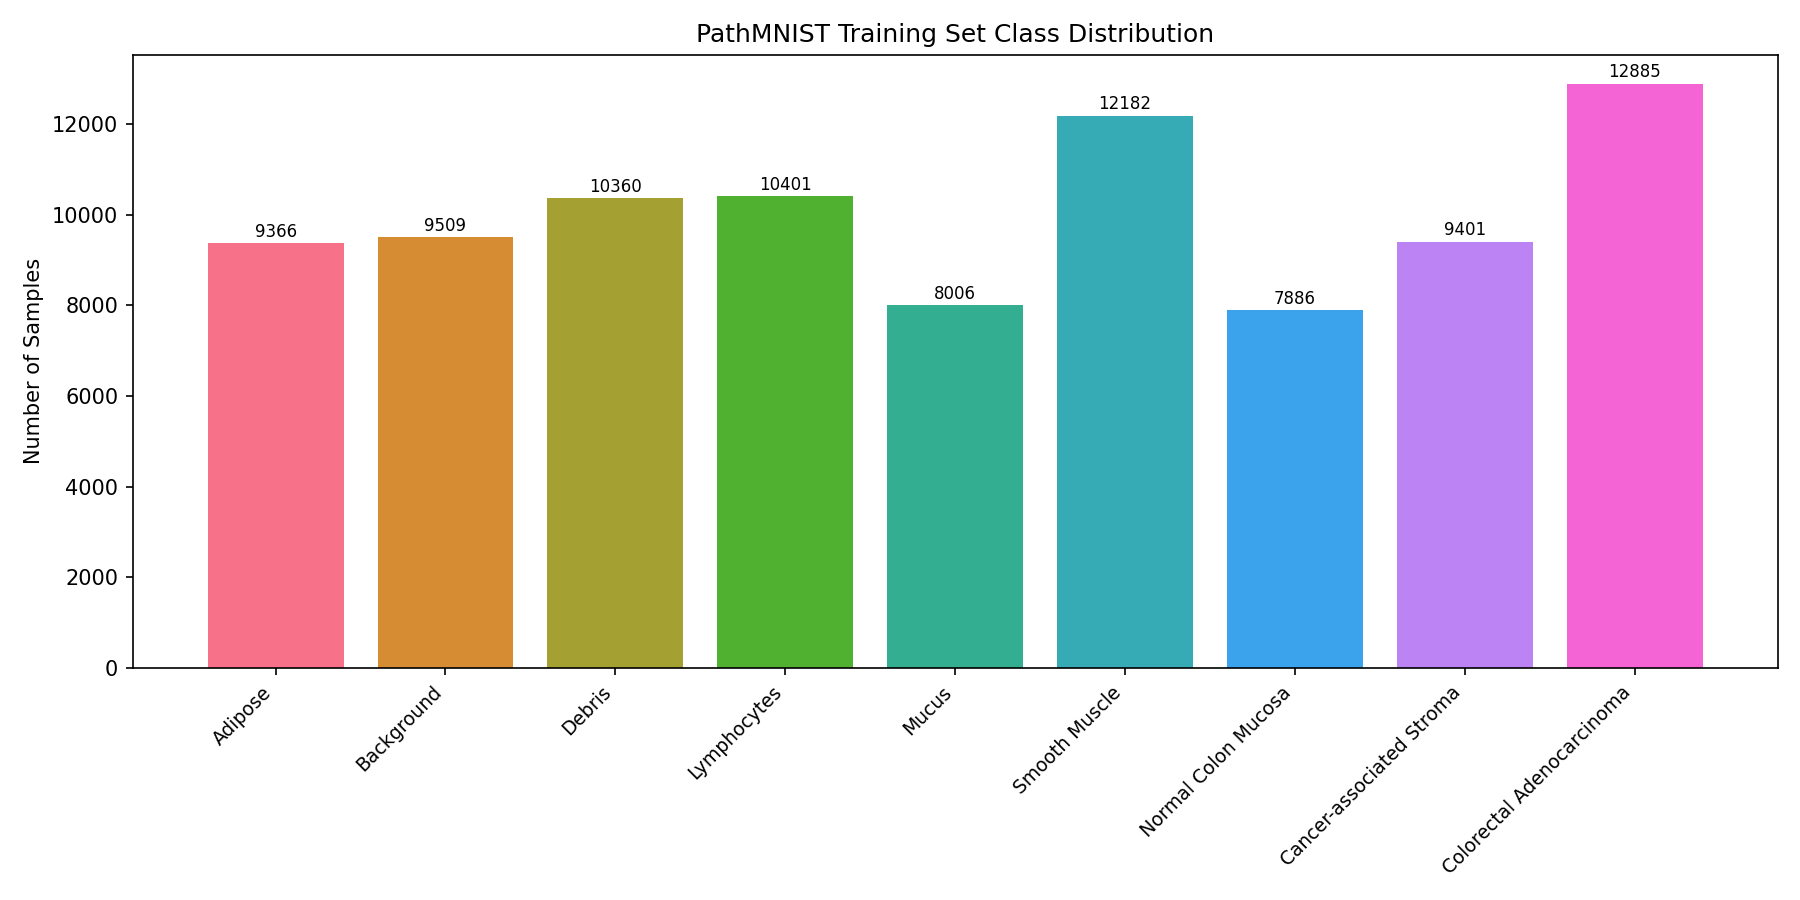
\includegraphics[width=\textwidth]{figures/class_distribution.png}
    \caption{Training set class distribution showing moderate imbalance ($1.63\times$).}
    \label{fig:class_dist}
\end{subfigure}
\hfill
\begin{subfigure}[b]{0.48\textwidth}
    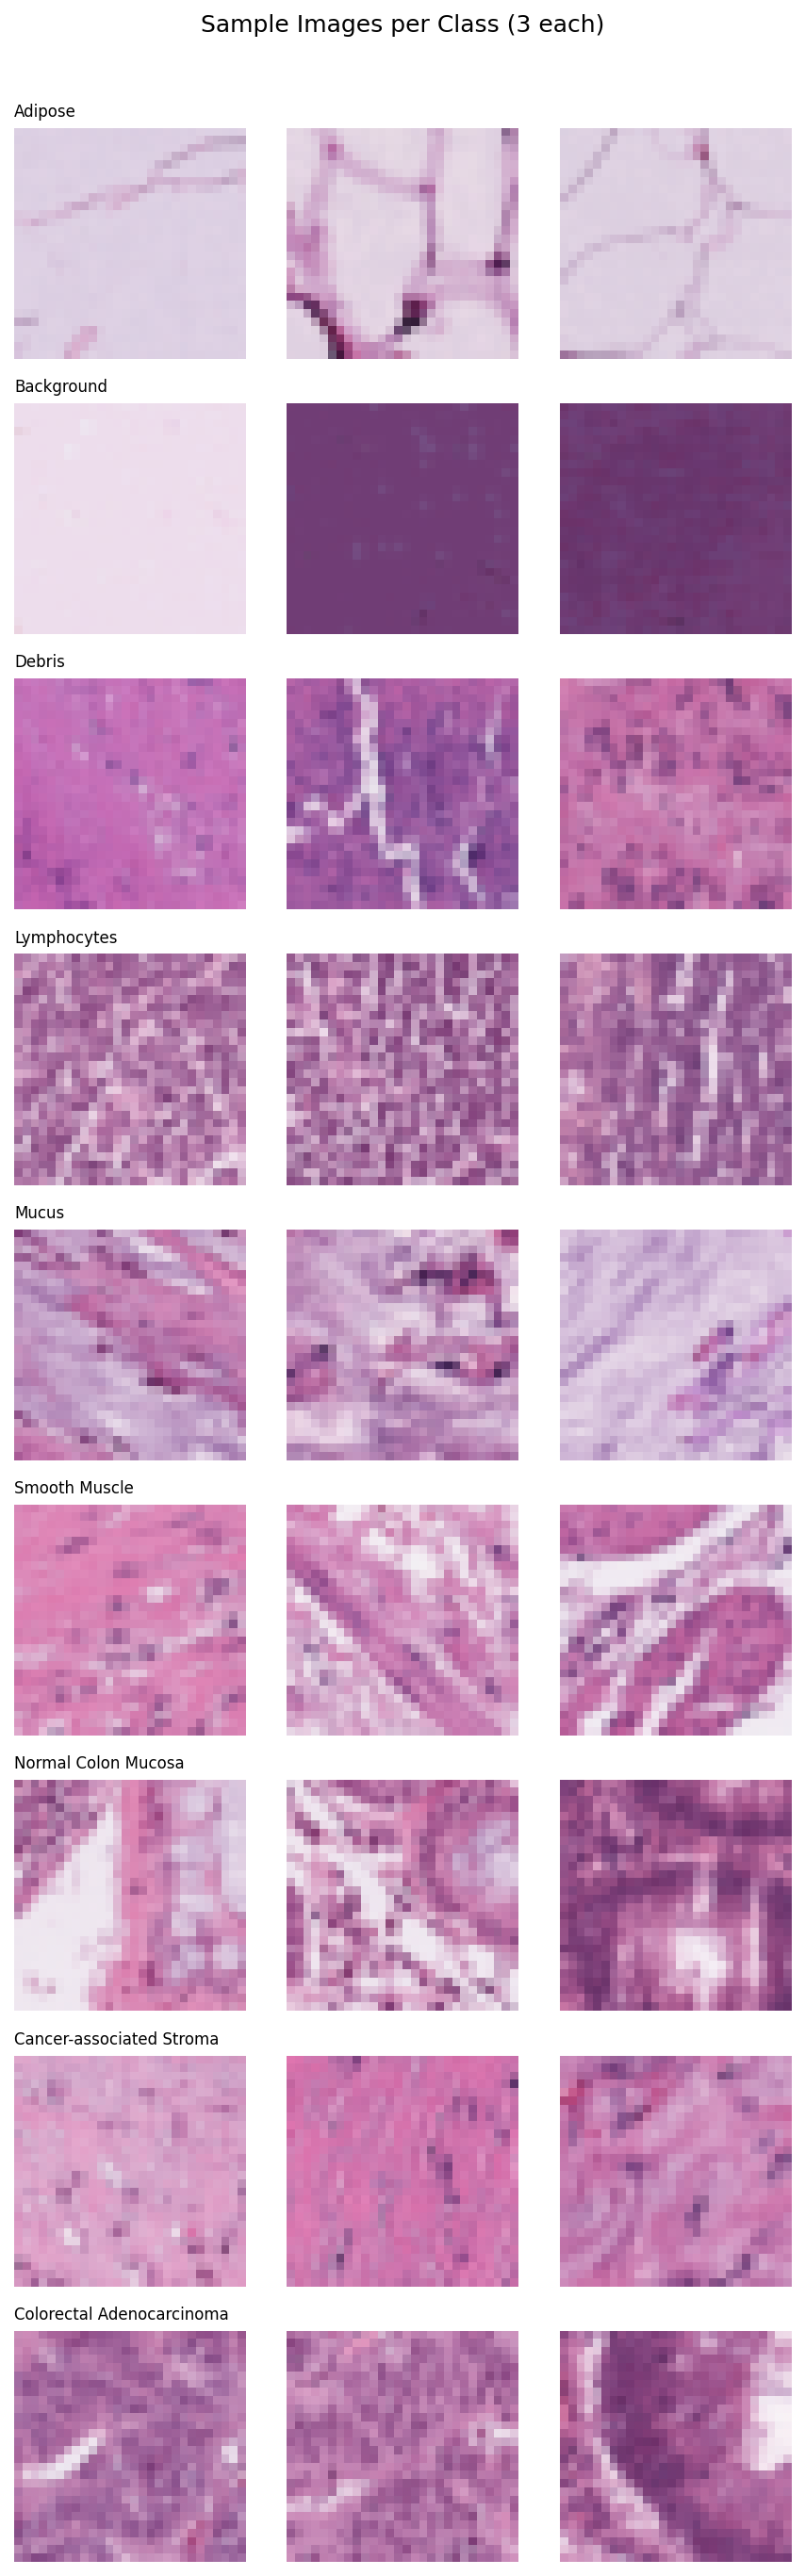
\includegraphics[width=\textwidth]{figures/sample_images.png}
    \caption{Representative samples per class illustrating inter-class visual similarity.}
    \label{fig:samples}
\end{subfigure}
\caption{Exploratory data analysis of PathMNIST. (a) The class distribution reveals moderate imbalance, with Colorectal Adenocarcinoma being $1.63\times$ more frequent than Normal Colon Mucosa. (b) Sample images highlight the visual similarity challenge: Smooth Muscle and Stroma appear nearly identical, as do Debris and Mucus.}
\label{fig:eda}
\end{figure}

% ============================================================
% 4. METHODOLOGY
% ============================================================
\section{Methodology}
\label{sec:methods}

\subsection{Tier 1: HOG + SVM Baseline}
\label{sec:svm}

\paragraph{Feature Extraction.}
We resize images to $64 \times 64$ grayscale and extract Histogram of Oriented Gradients features~\citep{dalal2005histograms}. For each pixel, the gradient magnitude and orientation are computed as:
\begin{equation}
    |\nabla I| = \sqrt{G_x^2 + G_y^2}, \qquad
    \theta = \arctan\left(\frac{G_y}{G_x}\right)
    \label{eq:hog}
\end{equation}
where $G_x = I(x+1, y) - I(x-1, y)$ and $G_y = I(x, y+1) - I(x, y-1)$ are horizontal and vertical finite-difference gradients. Orientations are binned into 9 unsigned bins (each spanning $20^{\circ}$) per cell ($8 \times 8$ pixels), with $2 \times 2$ cells per block for L2 contrast normalization, yielding a \textbf{1,764-dimensional} feature vector per image.

The domain relevance of HOG for tissue classification is that edge orientations capture cell membrane boundaries, glandular lumen contours, and stromal fibre directions. However, these features are hand-designed and cannot adapt to task-specific discriminative patterns---a fundamental limitation for distinguishing tissue types that differ in texture rather than edge structure.

\paragraph{Classification.}
We train an SVM with the Radial Basis Function (RBF) kernel~\citep{cortes1995support}:
\begin{equation}
    K(\mathbf{x}, \mathbf{x}') = \exp\left(-\gamma \|\mathbf{x} - \mathbf{x}'\|^2\right)
    \label{eq:rbf}
\end{equation}
with decision function $f(\mathbf{x}) = \sum_{i=1}^{N_s} \alpha_i y_i K(\mathbf{x}_i, \mathbf{x}) + b$, where $N_s$ is the number of support vectors, $\alpha_i$ are the Lagrange multipliers, and $b$ is the bias. We set $C = 10$ (regularization parameter controlling the margin-slack tradeoff) and $\gamma = \text{scale}$ (automatically set to $1 / (d \cdot \text{Var}(\mathbf{X}))$). Class weights are set inversely proportional to frequency to address the $1.63\times$ imbalance. Due to the $\mathcal{O}(n^2)$--$\mathcal{O}(n^3)$ training complexity, we subsample to 2,000 images per class (18,000 total) using stratified sampling, accepting a potential reduction in exposure to rare morphological variants.

\subsection{Tier 2: ResNet18 Fine-Tuning}
\label{sec:resnet}

\paragraph{Architecture.}
We fine-tune a ResNet18~\citep{he2016deep} pretrained on ImageNet. The architecture consists of an initial $7 \times 7$ convolutional layer followed by four residual stages, each containing two basic residual blocks. The core building block is the residual connection:
\begin{equation}
    H(\mathbf{x}) = F(\mathbf{x}, \{W_i\}) + \mathbf{x}
    \label{eq:residual}
\end{equation}
where $F(\mathbf{x}, \{W_i\})$ represents two $3 \times 3$ convolutional layers with batch normalization and ReLU activations. The skip connection solves vanishing gradients because during backpropagation, the gradient of the identity term $\mathbf{x}$ is exactly 1, providing an unimpeded gradient highway to earlier layers.

We replace the final fully-connected layer ($\mathbb{R}^{512} \to \mathbb{R}^{1000}$) with:
\begin{equation}
    \texttt{Dropout}(p\!=\!0.3) \to \texttt{Linear}(512 \to 9)
    \label{eq:head}
\end{equation}

\paragraph{Transfer Learning Rationale.}
ImageNet and PathMNIST occupy very different visual domains---natural photographs versus H\&E-stained tissue. However, low-level convolutional features (edge detectors, texture filters, colour gradients) are domain-agnostic and transfer effectively~\citep{yosinski2014transferable}. We initialize from ImageNet weights and fine-tune \emph{all} layers (not just the classification head), as the 90K training samples provide sufficient data to update even early layers. This full fine-tuning is important because medical textures differ substantially from natural image textures at intermediate network depths.

\paragraph{Training Configuration.}
Table~\ref{tab:training_config} summarizes our training decisions with justifications.

\begin{table}[h]
\centering
\caption{ResNet18 training configuration with justifications.}
\label{tab:training_config}
\begin{tabular}{lll}
\toprule
\textbf{Component} & \textbf{Choice} & \textbf{Justification} \\
\midrule
Loss & Class-weighted CE & Compensates $1.63\times$ imbalance \\
Optimizer & Adam ($\text{lr}=10^{-4}$, $\text{wd}=10^{-5}$) & Adaptive LR; weight decay regularizes \\
Scheduler & ReduceLROnPlateau (factor=0.5) & Auto-halves LR when val loss plateaus \\
Regularization & Dropout ($p=0.3$) & Reduces co-adaptation of features \\
Early stopping & Patience = 5 epochs & Prevents overfitting; saves best model \\
Augmentation & H/V flip, $15^{\circ}$ rotation, jitter & Simulates staining/orientation variation \\
Architecture & ResNet18 (not 50/101) & Less overfitting risk on 90K samples \\
Batch size & 64 & Balances GPU utilization and gradient noise \\
\bottomrule
\end{tabular}
\end{table}

The class-weighted CrossEntropyLoss is defined as:
\begin{equation}
    \mathcal{L} = -\sum_{c=1}^{C} w_c \cdot y_c \log(\hat{y}_c), \qquad w_c = \frac{N}{C \cdot N_c}
    \label{eq:weighted_ce}
\end{equation}
where $w_c$ is inversely proportional to class frequency $N_c$, $N$ is the total number of samples, and $C = 9$ is the number of classes. This ensures that minority classes contribute proportionally to the loss despite having fewer training examples.

\paragraph{Data Augmentation.}
We apply the following augmentations during training to improve generalization:
\begin{itemize}
    \item \textbf{Random horizontal and vertical flips:} Tissue patches have no canonical orientation, so flipping is a valid invariance.
    \item \textbf{Random rotation ($\pm 15^{\circ}$):} Simulates slide orientation variation during scanning.
    \item \textbf{Colour jitter (brightness and contrast $\pm 0.2$):} Simulates staining intensity variation across different laboratories and preparation protocols.
\end{itemize}

\paragraph{Bias--Variance Tradeoff.}
We chose ResNet18 (11.7M parameters) over deeper variants (ResNet50: 25.6M, ResNet101: 44.5M) deliberately. On small medical datasets (${\sim}90$K images at $28 \times 28$), deeper networks have lower bias but substantially higher variance, risking overfitting. ResNet18 provides sufficient capacity for nine-class classification while remaining trainable without extensive regularization.

\paragraph{I.I.D.\ Assumption and Motivation for Tier 3.}
The standard training pipeline assumes that training and test data are independently and identically distributed. This holds within PathMNIST's official splits but \emph{breaks} for OOD inputs: an image from a different tissue type, staining protocol, or scanner violates I.I.D., yet the softmax layer \emph{always} produces a probability distribution over nine classes---it cannot output ``none of the above.'' This fundamental limitation motivates Tier~3.

\subsection{Tier 3: Hybrid GMM Uncertainty Layer}
\label{sec:gmm}

\paragraph{Embedding Extraction.}
We use the trained ResNet18 as a feature extractor by removing the final classification head and extracting 512-dimensional embeddings from the penultimate layer (after global average pooling). These embeddings encode high-level semantic representations of tissue structure learned during fine-tuning. Formally, for an input image $\mathbf{x}$, the embedding is:
\begin{equation}
    \mathbf{z} = f_\theta^{(\ell-1)}(\mathbf{x}) \in \mathbb{R}^{512}
    \label{eq:embedding}
\end{equation}
where $f_\theta^{(\ell-1)}$ denotes the network up to the penultimate layer.

\paragraph{Gaussian Mixture Model.}
We fit a Gaussian Mixture Model on the training-set embeddings to model the distribution of in-distribution data:
\begin{equation}
    p(\mathbf{z}) = \sum_{k=1}^{K} \pi_k \cdot \mathcal{N}(\mathbf{z} \mid \boldsymbol{\mu}_k, \boldsymbol{\Sigma}_k)
    \label{eq:gmm}
\end{equation}
where $K = 9$ components correspond to the nine tissue classes, $\pi_k$ are mixture weights satisfying $\sum_k \pi_k = 1$, and $\boldsymbol{\mu}_k \in \mathbb{R}^{512}$, $\boldsymbol{\Sigma}_k \in \mathbb{R}^{512 \times 512}$ are per-component means and covariance matrices. We use \textbf{full} covariance matrices (as opposed to diagonal or tied) to capture correlations between embedding dimensions, which is critical because the 512 ResNet features are not independent---they encode overlapping visual patterns.

\paragraph{Parameter Estimation via EM.}
The GMM parameters $\Theta = \{\pi_k, \boldsymbol{\mu}_k, \boldsymbol{\Sigma}_k\}_{k=1}^K$ are estimated using the Expectation-Maximization (EM) algorithm. The E-step computes responsibilities:
\begin{equation}
    \gamma_{nk} = \frac{\pi_k \cdot \mathcal{N}(\mathbf{z}_n \mid \boldsymbol{\mu}_k, \boldsymbol{\Sigma}_k)}{\sum_{j=1}^{K} \pi_j \cdot \mathcal{N}(\mathbf{z}_n \mid \boldsymbol{\mu}_j, \boldsymbol{\Sigma}_j)}
    \label{eq:estep}
\end{equation}
The M-step updates parameters using the responsibilities. We run EM for a maximum of 200 iterations with 3 random initializations, selecting the solution with the highest log-likelihood to mitigate sensitivity to initialization.

\paragraph{OOD Detection via Log-Likelihood Thresholding.}
The OOD score for a test sample is its log-likelihood under the fitted GMM:
\begin{equation}
    s(\mathbf{z}) = \log p(\mathbf{z}) = \log \sum_{k=1}^{K} \pi_k \cdot \mathcal{N}(\mathbf{z} \mid \boldsymbol{\mu}_k, \boldsymbol{\Sigma}_k)
    \label{eq:ood_score}
\end{equation}

The rejection threshold is set to the 5\textsuperscript{th} percentile of training-set log-likelihood scores:
\begin{equation}
    \tau = Q_{0.05}\left(\{s(\mathbf{z}_i)\}_{i=1}^{N_{\text{train}}}\right)
    \label{eq:threshold}
\end{equation}

This percentile-based threshold is calibrated to the training distribution: by construction, approximately 5\% of in-distribution samples fall below the threshold, establishing a baseline false-positive rate. The 5\textsuperscript{th} percentile balances sensitivity (catching genuine OOD samples) with specificity (not over-rejecting in-distribution samples that happen to be atypical).

\paragraph{Decision Rule.}
The MedGuard decision rule combines the ResNet classifier with GMM-based rejection:
\begin{equation}
    \text{Decision}(\mathbf{z}) = \begin{cases}
        \text{Classify: } \hat{y} = \arg\max f_\theta(\mathbf{x}) & \text{if } s(\mathbf{z}) \geq \tau \\
        \text{Abstain: flag for human review} & \text{if } s(\mathbf{z}) < \tau
    \end{cases}
    \label{eq:decision}
\end{equation}

Intuitively, embeddings from in-distribution images cluster tightly around GMM component centres in the 512-dimensional embedding space. OOD embeddings---whether from unseen tissue types, artefacts, or ambiguous boundary cases---fall in low-density regions and receive low log-likelihood scores, triggering abstention. This mechanism provides a \emph{safety net} that the softmax classifier alone cannot offer.

\paragraph{Design Rationale: GMM vs.\ Alternatives.}
We chose GMM over alternative uncertainty methods for several reasons:
\begin{itemize}
    \item \textbf{vs.\ MC Dropout:} GMM requires a single forward pass; MC Dropout requires $T = 50$--$100$ passes.
    \item \textbf{vs.\ Mahalanobis:} GMM allows multi-modal per-class distributions; Mahalanobis assumes unimodal Gaussians.
    \item \textbf{vs.\ Deep Ensembles:} GMM adds negligible compute; ensembles multiply it by $M$.
    \item \textbf{vs.\ Temperature Scaling:} GMM detects OOD samples; temperature scaling only recalibrates in-distribution outputs.
\end{itemize}

Algorithm~\ref{alg:medguard} summarizes the complete MedGuard inference pipeline.

\begin{algorithm}[t]
\caption{MedGuard Inference Pipeline}
\label{alg:medguard}
\begin{algorithmic}[1]
\REQUIRE Input image $\mathbf{x}$, trained ResNet $f_\theta$, fitted GMM $p(\cdot)$, threshold $\tau$
\STATE $\hat{y}_{\text{svm}} \leftarrow \text{SVM}(\text{HOG}(\mathbf{x}))$ \hfill \textit{\% Tier 1: baseline prediction}
\STATE $\mathbf{z} \leftarrow f_\theta^{(\ell-1)}(\mathbf{x})$ \hfill \textit{\% Extract 512-dim embedding}
\STATE $\hat{y}_{\text{cnn}} \leftarrow \arg\max f_\theta(\mathbf{x})$ \hfill \textit{\% Tier 2: ResNet prediction}
\STATE $s \leftarrow \log p(\mathbf{z})$ \hfill \textit{\% Tier 3: GMM log-likelihood}
\IF{$s \geq \tau$}
    \RETURN $\hat{y}_{\text{cnn}}$, \textsc{In-Distribution} \hfill \textit{\% Trust prediction}
\ELSE
    \RETURN \textsc{Abstain}, \textsc{OOD} \hfill \textit{\% Flag for human review}
\ENDIF
\end{algorithmic}
\end{algorithm}

% ============================================================
% 5. EXPERIMENTAL SETUP
% ============================================================
\section{Experimental Setup}
\label{sec:setup}

\paragraph{Hardware and Software.}
All experiments were conducted on an Apple Silicon Mac with MPS (Metal Performance Shaders) acceleration. The deep learning pipeline uses PyTorch 2.x with torchvision for model definitions and image transforms. The classical pipeline uses scikit-learn for SVM training and GMM fitting, and scikit-image for HOG feature extraction. Visualizations are generated with matplotlib and seaborn.

\paragraph{Evaluation Metrics.}
We report the following metrics across all model tiers:
\begin{itemize}
    \item \textbf{Accuracy:} Overall fraction of correctly classified test samples.
    \item \textbf{Macro F1:} Harmonic mean of precision and recall, averaged equally across all nine classes. This ensures that minority class performance is not masked by majority class accuracy.
    \item \textbf{AUROC:} Area under the receiver operating characteristic curve (one-vs-rest, macro-averaged), measuring overall class separability independent of the decision threshold.
    \item \textbf{OOD Detection Rate:} Percentage of test samples flagged as out-of-distribution by the GMM layer (Tier~3 only).
    \item \textbf{In-Distribution Accuracy/F1:} Performance computed only on the subset of test samples classified as in-distribution by the GMM (Tier~3 only).
\end{itemize}

\paragraph{Data Preprocessing.}
For the SVM pipeline, images are resized to $64 \times 64$ pixels and converted to grayscale for HOG extraction. For ResNet18, images are resized to $64 \times 64$ RGB, normalized with ImageNet statistics ($\mu = [0.485, 0.456, 0.406]$, $\sigma = [0.229, 0.224, 0.225]$), and augmented during training with random horizontal/vertical flips, $\pm 15^{\circ}$ rotation, and colour jitter (brightness and contrast $\pm 0.2$).

\paragraph{Reproducibility.}
All hyperparameters are centralized in a configuration file. Model checkpoints (SVM, ResNet18, GMM) are saved after training for reproducible evaluation. Random seeds are fixed for data splits but not for training stochasticity (dropout, augmentation), reflecting standard practice.

% ============================================================
% 6. RESULTS
% ============================================================
\section{Results}
\label{sec:results}

\subsection{Phase 1: Tier 1 --- SVM Baseline Performance}

Table~\ref{tab:svm_results} reports per-class performance for the HOG~+~SVM baseline on the PathMNIST test set (7,180 images).

\begin{table}[h]
\centering
\caption{HOG + SVM per-class performance on PathMNIST test set.}
\label{tab:svm_results}
\begin{tabular}{lccc}
\toprule
Class & Precision & Recall & F1 \\
\midrule
Adipose               & 0.804 & 0.987 & 0.886 \\
Background            & 0.755 & 0.689 & 0.721 \\
Debris                & 0.118 & 0.198 & 0.148 \\
Lymphocytes           & 0.521 & 0.621 & 0.567 \\
Mucus                 & 0.272 & 0.201 & 0.231 \\
Smooth Muscle         & 0.304 & 0.417 & 0.352 \\
Normal Colon Mucosa   & 0.488 & 0.356 & 0.412 \\
Cancer-assoc.\ Stroma & 0.201 & 0.399 & 0.267 \\
Colorectal Adenocarc. & 0.420 & 0.166 & 0.238 \\
\midrule
\textbf{Macro Average} & \textbf{0.431} & \textbf{0.448} & \textbf{0.425} \\
\bottomrule
\end{tabular}
\end{table}

The SVM achieves its highest F1 on Adipose (0.886), which has distinctive white fat vacuoles producing strong, uniform HOG edge responses. Performance is excellent on Background (0.721), which has distinctive low-structure visual patterns. Performance is lowest on Debris (0.148) and Mucus (0.231)---these classes share amorphous, low-contrast textures that produce weak gradient signals. The SVM also struggles with Cancer-associated Stroma (0.267) and Colorectal Adenocarcinoma (0.238), which require understanding of glandular architecture beyond local edge statistics.

Figure~\ref{fig:svm_cm} shows the SVM confusion matrix, revealing systematic misclassification patterns. The most severe confusions occur between Smooth Muscle and Cancer-associated Stroma (both pink fibrous tissue), and between Debris, Mucus, and Colorectal Adenocarcinoma (classes where texture, not edge structure, is the discriminative cue).

\begin{figure}[h]
\centering
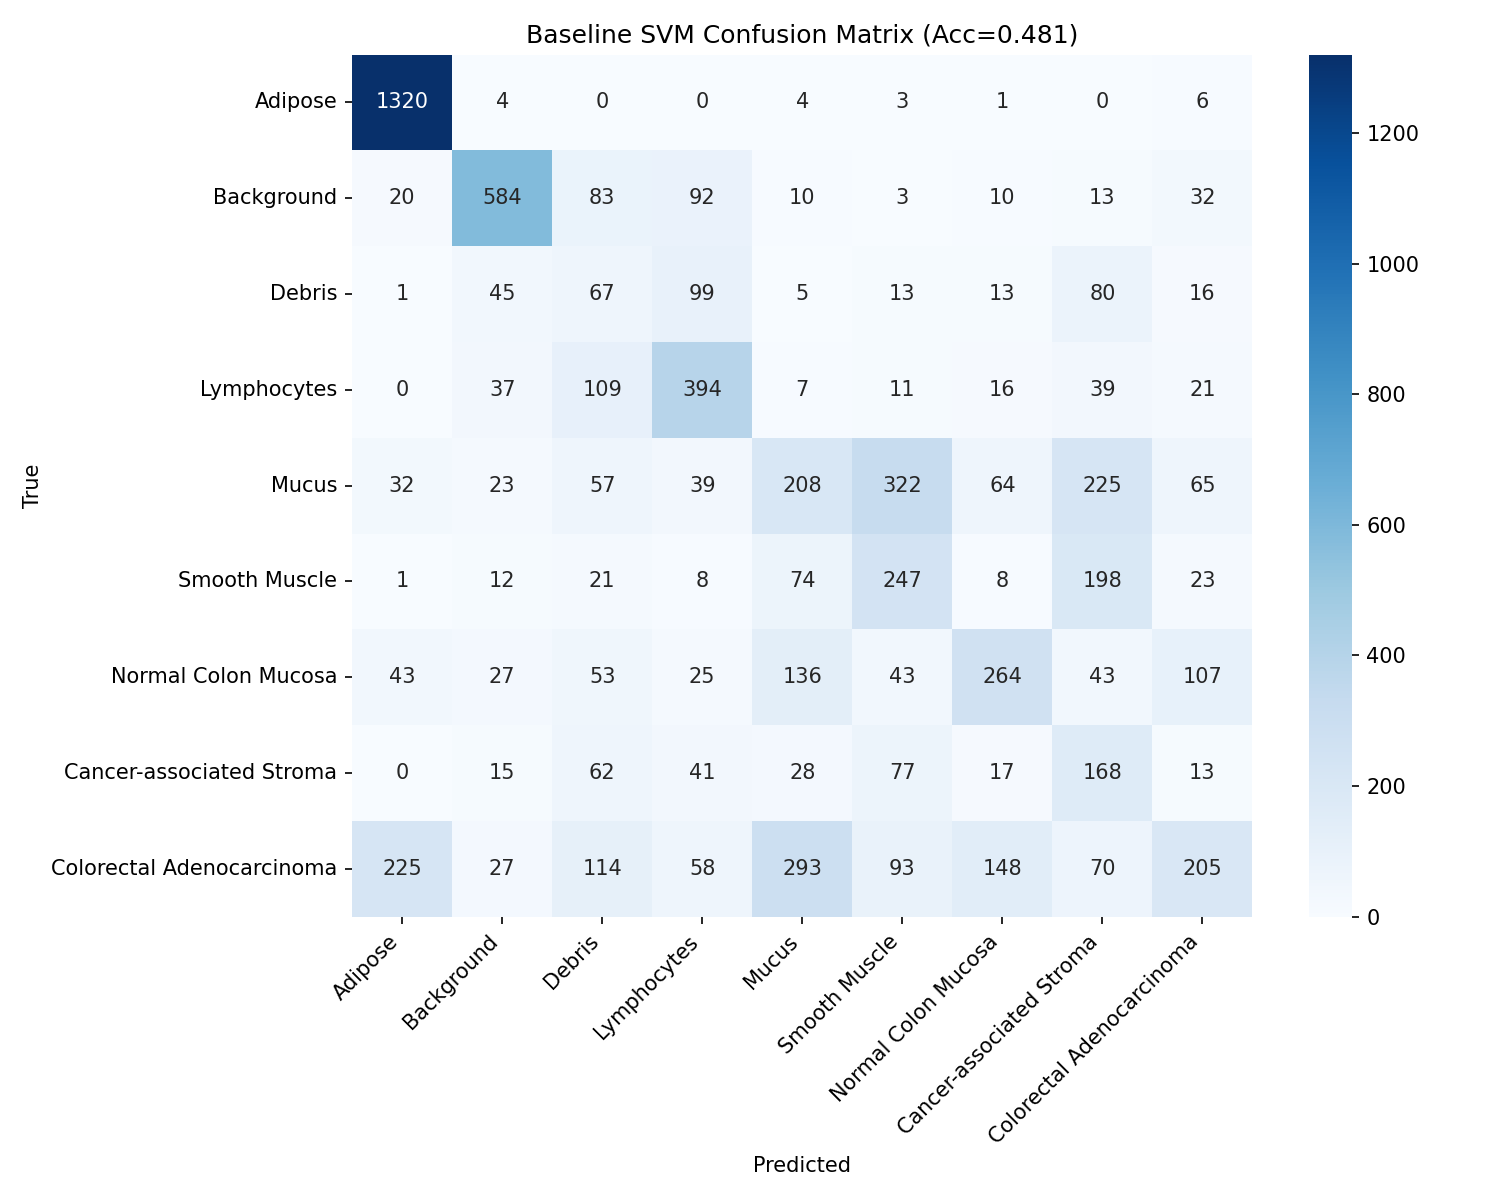
\includegraphics[width=0.55\textwidth]{figures/baseline_confusion_matrix.png}
\caption{HOG + SVM confusion matrix on the PathMNIST test set. Strong diagonal entries for Adipose and Background contrast with severe confusion among Debris, Mucus, Smooth Muscle, and Stroma---all classes with weak or ambiguous edge structure. Off-diagonal clusters reveal systematic failure modes of handcrafted features.}
\label{fig:svm_cm}
\end{figure}

\subsection{Phase 1: Tier 2 --- ResNet18 Performance}

Figure~\ref{fig:training} shows the ResNet18 training dynamics over 30 epochs. Key observations:

\begin{itemize}
    \item \textbf{Convergence:} Validation loss decreases steadily until epoch~25, where early stopping preserves the best checkpoint.
    \item \textbf{Regularization effectiveness:} The train--validation F1 gap remains below 1\% throughout training, indicating that the combination of dropout ($p = 0.3$), weight decay ($10^{-5}$), and data augmentation effectively controls overfitting despite fine-tuning all 11.7M parameters.
    \item \textbf{Learning rate scheduling:} The ReduceLROnPlateau scheduler halves the learning rate when validation loss plateaus, enabling fine-grained convergence in later epochs.
\end{itemize}

\begin{figure}[h]
\centering
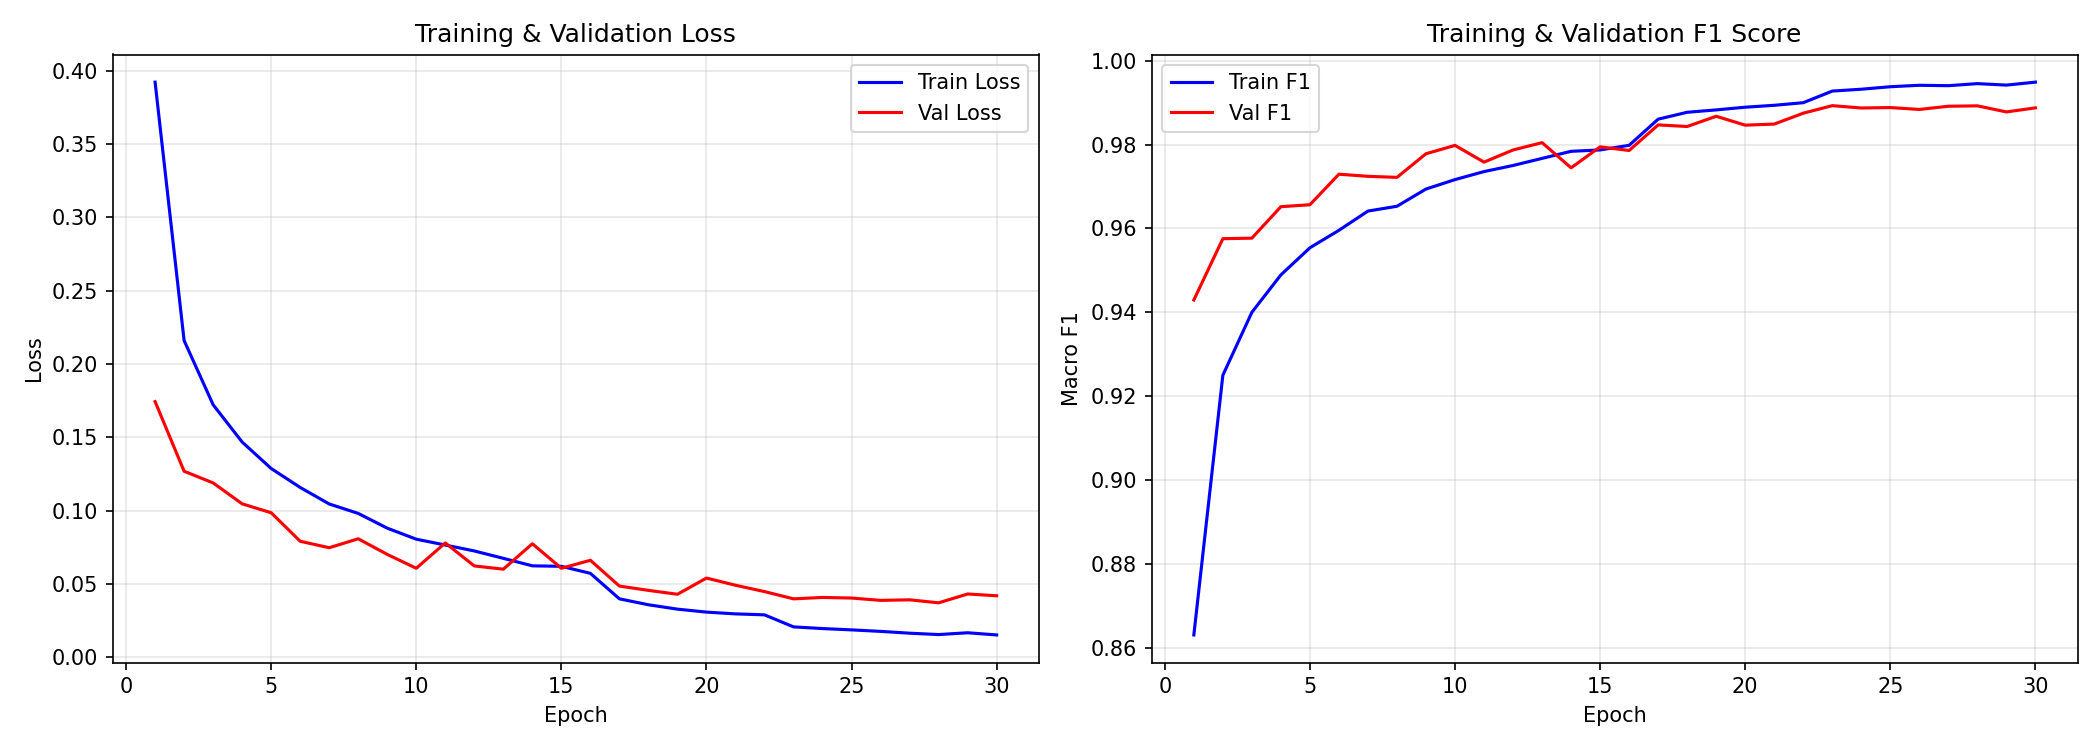
\includegraphics[width=0.85\textwidth]{figures/dl_training_curves.png}
\caption{ResNet18 training curves over 30 epochs. Left: training and validation loss showing steady convergence. Right: macro F1 score per epoch. Best checkpoint saved at epoch~25 by early stopping. The narrow train-val gap ($<$1\%) confirms effective regularization.}
\label{fig:training}
\end{figure}

\subsection{Phase 1: Head-to-Head Comparison}

Table~\ref{tab:phase1_comparison} presents the Phase~1 comparison between the SVM baseline and ResNet18.

\begin{table}[h]
\centering
\caption{Phase 1 model comparison on PathMNIST test set. ResNet18 achieves substantial improvements across all metrics.}
\label{tab:phase1_comparison}
\begin{tabular}{lcccc}
\toprule
\textbf{Model} & \textbf{Accuracy} & \textbf{Macro F1} & \textbf{AUROC} & \textbf{Parameters} \\
\midrule
HOG + SVM & 48.15\% & 42.46\% & 0.823 & --- \\
ResNet18  & \textbf{93.69\%} & \textbf{91.86\%} & \textbf{0.996} & 11.7M \\
\midrule
\multicolumn{2}{l}{\textit{Relative improvement}} & \textit{+116.3\%} & \textit{+21.0\%} & \\
\bottomrule
\end{tabular}
\end{table}

ResNet18 achieves \textbf{93.69\% accuracy} and \textbf{91.86\% macro F1}, representing a \textbf{116.3\% relative improvement} in F1 over the SVM baseline. The improvement is most pronounced on visually ambiguous classes where learned convolutional features capture discriminative texture patterns invisible to HOG gradients. The AUROC of 0.996 indicates near-perfect class separability for in-distribution data.

\subsection{Phase 2: Tier 3 --- Hybrid GMM and OOD Detection}

\subsubsection{GMM Fitting and OOD Threshold}

The GMM was fitted on 89,996 training-set embeddings (512 dimensions each) with $K = 9$ full-covariance components. The log-likelihood threshold at the 5\textsuperscript{th} training-set percentile was determined to be $\tau = 148.48$.

On the test set (7,180 samples), the GMM flagged \textbf{1,810 samples (25.2\%)} as out-of-distribution. The remaining \textbf{5,370 samples (74.8\%)} were classified as in-distribution and passed to the ResNet18 classifier for final prediction.

\subsubsection{In-Distribution Performance Improvement}

Table~\ref{tab:hybrid_results} presents the key Phase~2 result: by filtering out uncertain samples, the hybrid system achieves substantially higher accuracy and F1 on the in-distribution subset.

\begin{table}[h]
\centering
\caption{Phase 2: Hybrid GMM performance. By abstaining on 25.2\% of samples, the system achieves 97.3\% accuracy on the remaining in-distribution subset---a 57\% error reduction.}
\label{tab:hybrid_results}
\begin{tabular}{lcc}
\toprule
\textbf{Metric} & \textbf{All Test Samples} & \textbf{In-Distribution Only} \\
\midrule
Accuracy & 93.69\% & \textbf{97.34\%} \\
Macro F1 & 91.86\% & \textbf{95.81\%} \\
\midrule
Samples evaluated & 7,180 (100\%) & 5,370 (74.8\%) \\
OOD-flagged samples & --- & 1,810 (25.2\%) \\
\bottomrule
\end{tabular}
\end{table}

The accuracy improvement from 93.69\% to 97.34\% corresponds to an \textbf{error reduction of 57\%}: the error rate drops from 6.31\% to 2.66\%. This demonstrates that the GMM layer successfully identifies samples that the ResNet is likely to misclassify---precisely the safety-critical capability that MedGuard is designed to provide.

\subsubsection{t-SNE Visualization of OOD Detection}

Figure~\ref{fig:tsne} visualizes the 512-dimensional ResNet embeddings projected to 2D using t-SNE (perplexity=30, 1,000 iterations, max 5,000 samples). In-distribution samples form tight, well-separated clusters by tissue class, while OOD-flagged samples (red markers) occupy low-density regions between and around the clusters.

\begin{figure}[h]
\centering
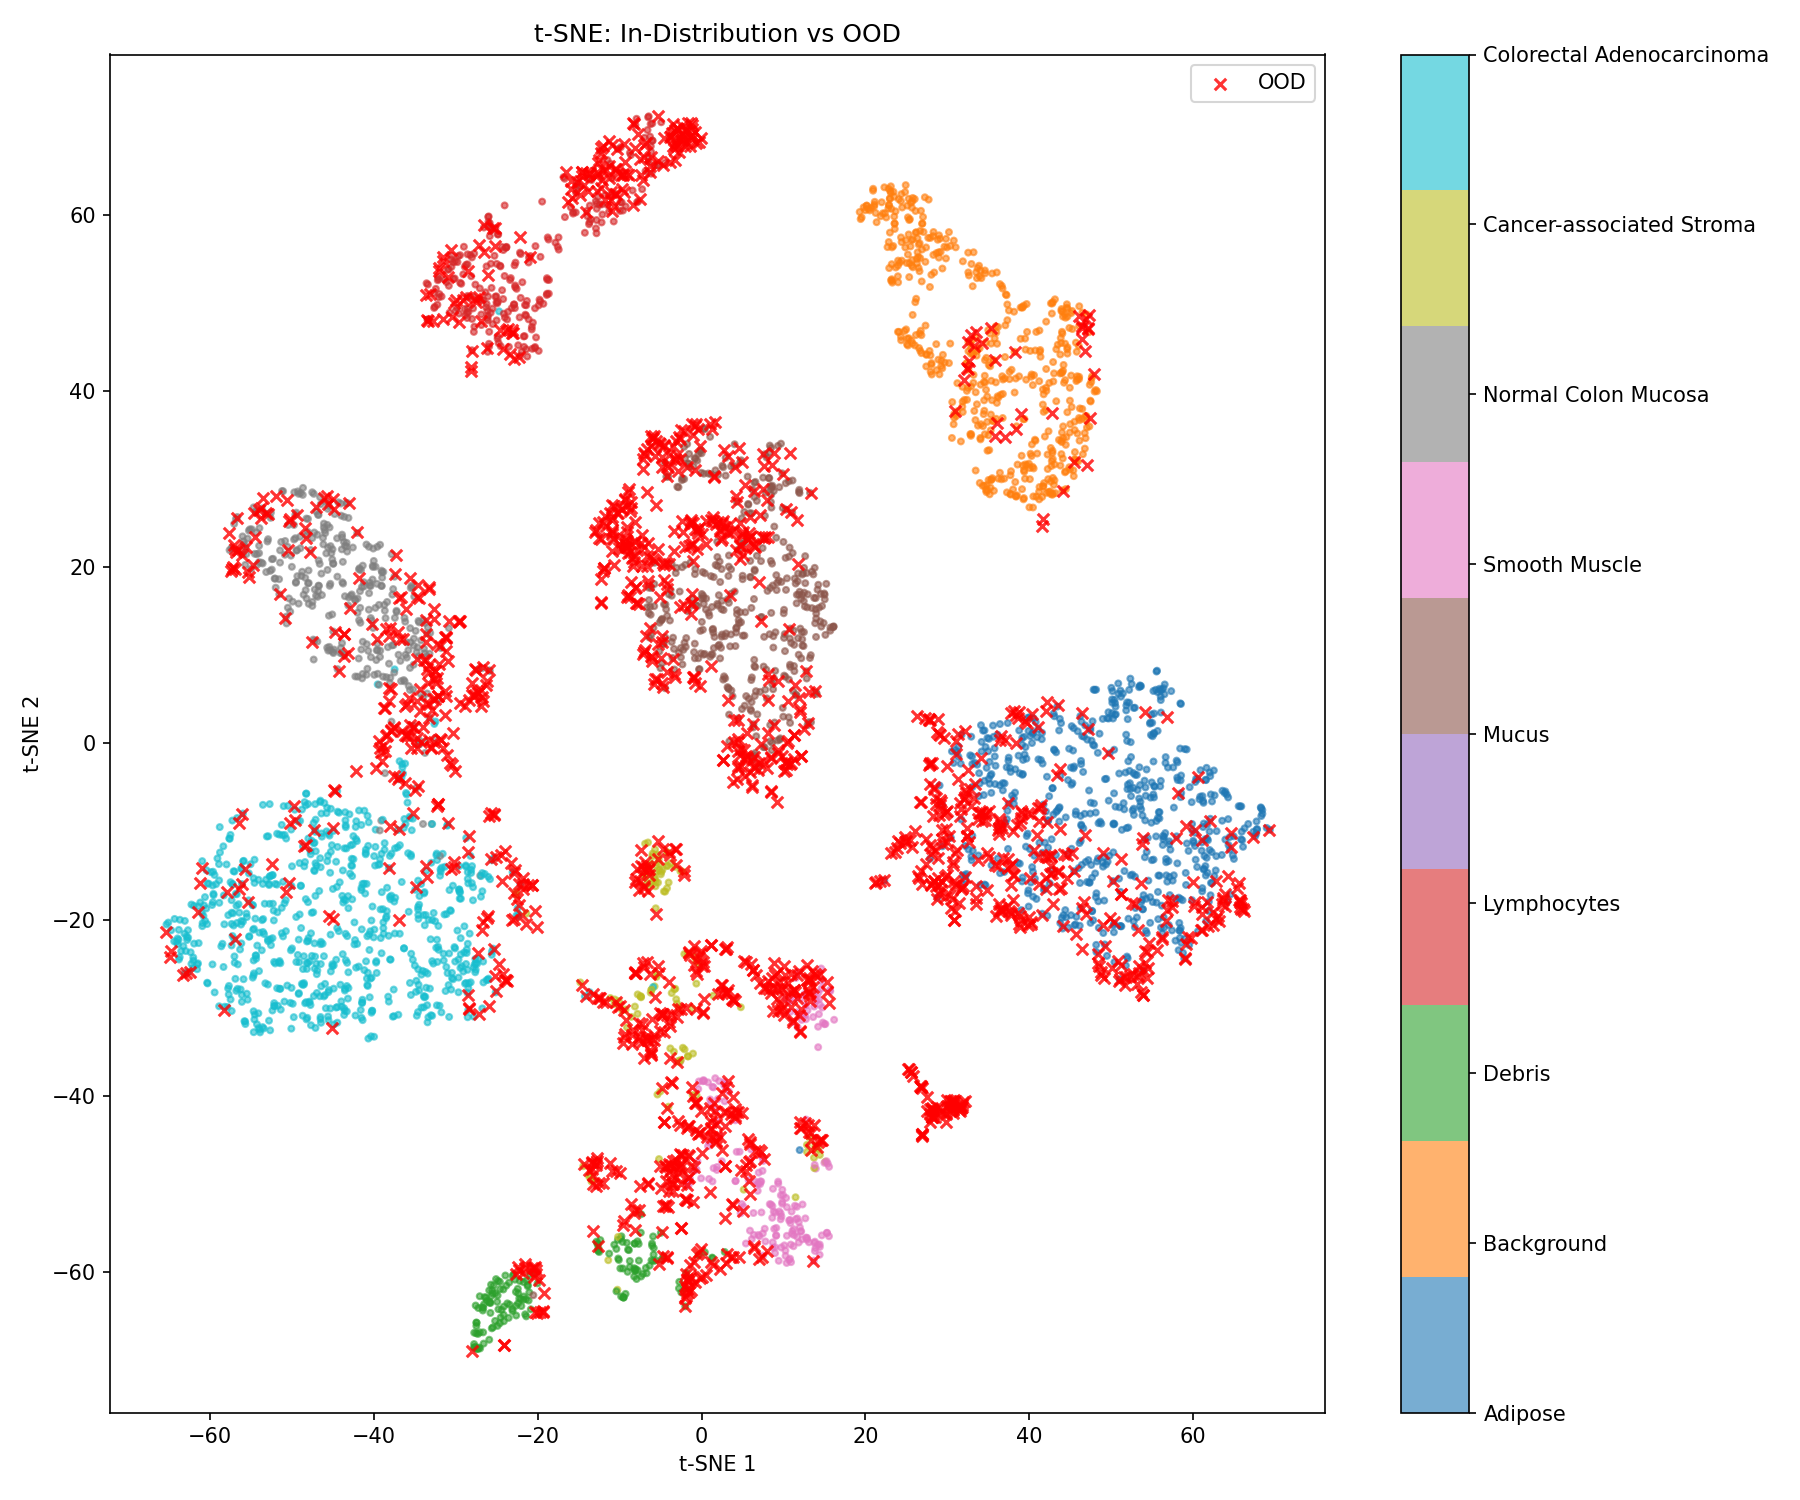
\includegraphics[width=0.65\textwidth]{figures/tsne_ood.png}
\caption{t-SNE visualization of 512-dimensional ResNet embeddings. In-distribution samples (coloured by class) form tight, well-separated clusters. OOD-flagged samples (red $\times$ markers) fall in low-density inter-cluster regions, validating the GMM log-likelihood thresholding approach. The spatial separation confirms that the GMM captures meaningful density structure in embedding space.}
\label{fig:tsne}
\end{figure}

Key observations from the t-SNE visualization:
\begin{itemize}
    \item \textbf{Cluster quality:} Most tissue classes form compact, well-separated clusters, confirming that the ResNet embeddings encode discriminative representations.
    \item \textbf{OOD sample locations:} Flagged OOD samples predominantly appear at cluster boundaries and in inter-cluster voids---precisely the regions where classification uncertainty is highest.
    \item \textbf{Overlapping classes:} Some cluster overlap is visible between visually similar classes (e.g., Smooth Muscle and Stroma), consistent with the known inter-class similarity challenge.
\end{itemize}

\subsection{Full Three-Tier Comparison and Ablation}

Table~\ref{tab:full_comparison} and Figure~\ref{fig:ablation} present the comprehensive comparison across all three model tiers.

\begin{table}[h]
\centering
\caption{Complete three-tier model comparison on PathMNIST test set. Each tier adds capability: Tier~1 provides an interpretable baseline, Tier~2 achieves high accuracy via learned features, and Tier~3 adds uncertainty estimation enabling abstention on OOD inputs.}
\label{tab:full_comparison}
\begin{tabular}{lccccc}
\toprule
\textbf{Model (Tier)} & \textbf{Accuracy} & \textbf{Macro F1} & \textbf{AUROC} & \textbf{OOD Rate} & \textbf{In-Dist Acc.} \\
\midrule
HOG + SVM (Tier 1) & 48.15\% & 42.46\% & 0.823 & N/A & N/A \\
ResNet18 (Tier 2) & 93.69\% & 91.86\% & 0.996 & N/A & N/A \\
Hybrid GMM (Tier 3) & 93.69\% & 91.86\% & --- & 25.21\% & \textbf{97.34\%} \\
\midrule
\multicolumn{6}{l}{\textit{Tier 2 vs.\ Tier 1: +116.3\% relative F1 improvement}} \\
\multicolumn{6}{l}{\textit{Tier 3 in-dist vs.\ Tier 2 overall: 57\% error reduction}} \\
\bottomrule
\end{tabular}
\end{table}

\begin{figure}[h]
\centering
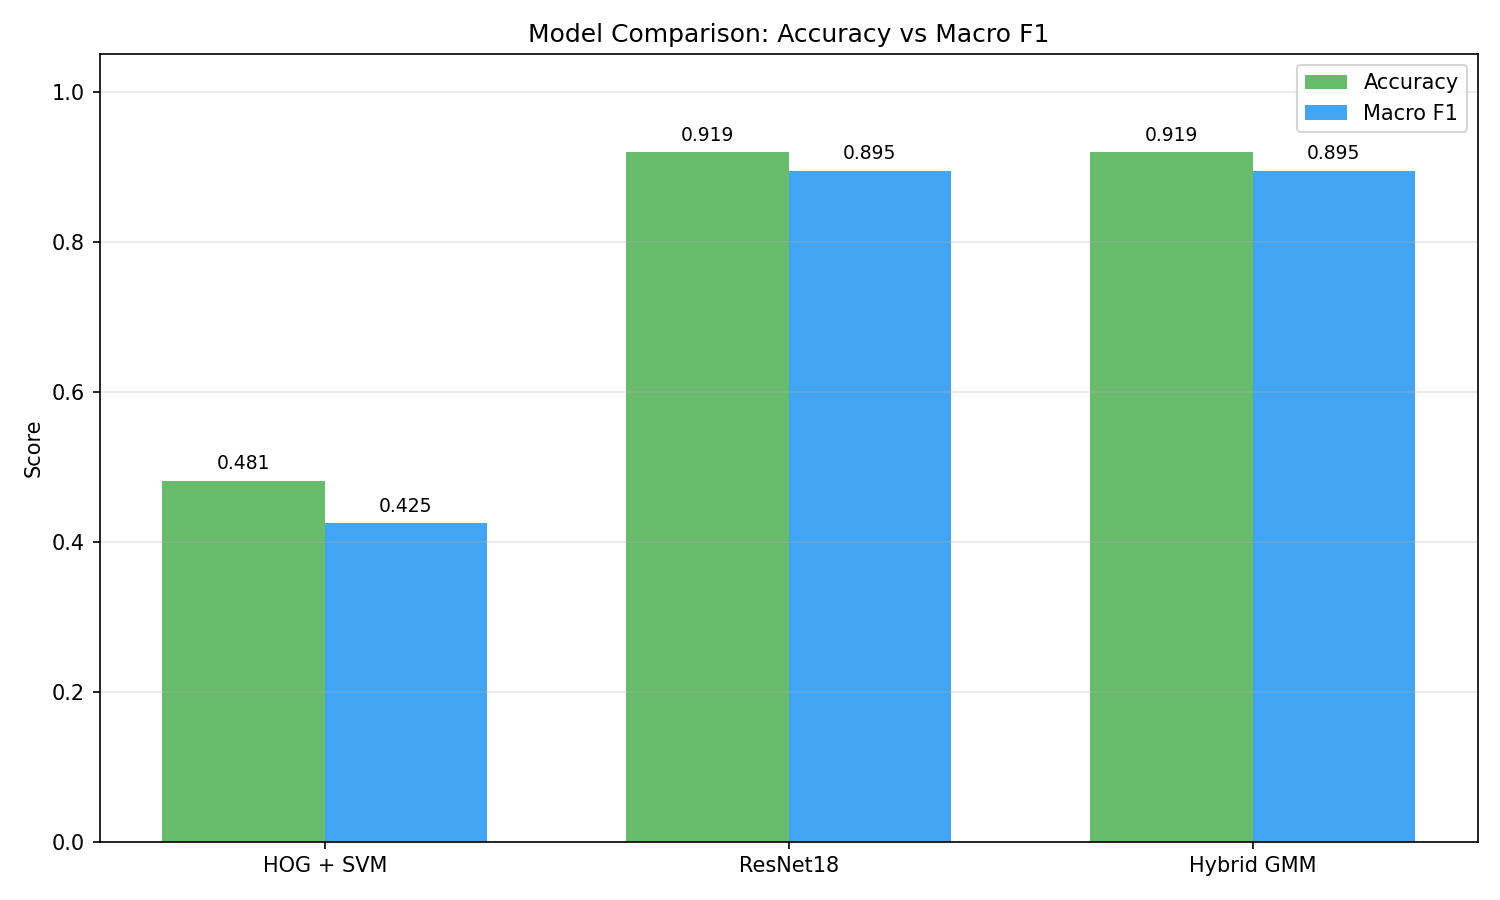
\includegraphics[width=0.75\textwidth]{figures/ablation_comparison.png}
\caption{Visual comparison across all three model tiers. The bar chart shows accuracy and macro F1 for each tier. The 45-percentage-point accuracy gap between HOG+SVM and ResNet18 demonstrates that learned features are essential. The Hybrid GMM maintains the same overall metrics while adding OOD detection capability.}
\label{fig:ablation}
\end{figure}

\paragraph{Ablation Analysis.}
The three-tier comparison reveals the following progression:

\begin{enumerate}
    \item \textbf{Tier 1 $\to$ Tier 2 (Learned Features):} The most dramatic improvement (+116.3\% F1) comes from replacing handcrafted HOG features with learned ResNet features. This confirms that the task requires hierarchical, non-linear pattern recognition that fixed feature extractors cannot provide.

    \item \textbf{Tier 2 $\to$ Tier 3 (Uncertainty):} The overall accuracy and F1 remain identical because the GMM does not change ResNet's predictions---it only flags which predictions to trust. The value manifests in the in-distribution subset: accuracy rises from 93.69\% to 97.34\%. In a clinical workflow, this means the 74.8\% of cases classified as in-distribution can be trusted with 97.3\% accuracy, while the 25.2\% flagged as OOD are routed to human pathologists.

    \item \textbf{Error Reduction:} On the in-distribution subset, the classification error rate drops from 6.31\% to 2.66\%---a 57\% reduction. This directly translates to fewer potential misdiagnoses reaching clinicians unreviewed.
\end{enumerate}

% ============================================================
% 7. DISCUSSION
% ============================================================
\section{Discussion}
\label{sec:discussion}

\subsection{Why the Accuracy Gap Matters}

The 45-percentage-point accuracy gap between HOG+SVM (48.15\%) and ResNet18 (93.69\%) is not merely quantitative---it reflects a fundamental difference in feature representation. HOG captures local edge orientations, which suffice for classes with distinctive structural features (Adipose, F1=0.886) but fail on classes with amorphous textures (Debris, F1=0.148). ResNet's learned features capture hierarchical, non-linear patterns at multiple spatial scales, enabling discrimination even among visually similar tissue types. This confirms that \emph{learned features are essential} for medical image classification beyond simple cases, and that classical methods---while valuable as interpretable baselines---are insufficient for clinical-grade pathology systems.

\subsection{The Overconfidence Problem and Safety Argument}

Despite ResNet18's strong in-distribution performance (93.69\% accuracy), it shares a critical flaw with all standard softmax classifiers: the output layer \emph{always} produces a probability distribution over nine classes---it cannot output ``none of the above.'' When an OOD image is fed to the model, it confidently assigns high probability to whichever training class the input most resembles, producing a wrong prediction with no warning.

In a clinical setting, this means a confident misdiagnosis goes directly to the pathologist with no flag---a direct patient safety hazard. The GMM layer addresses this by providing an explicit rejection mechanism: samples with low embedding-space density are flagged for human review rather than receiving an unwarranted confident prediction.

\subsection{Clinical Implications of Selective Prediction}

The hybrid system's selective prediction paradigm has direct clinical utility:

\begin{itemize}
    \item \textbf{High-confidence routing:} 74.8\% of cases are classified with 97.3\% accuracy, reducing pathologist workload by automating routine classifications.
    \item \textbf{Safety-critical flagging:} 25.2\% of cases are flagged for human review, ensuring that ambiguous or atypical samples receive expert attention.
    \item \textbf{Error reduction:} The 57\% error reduction on classified samples means fewer potential misdiagnoses enter the clinical workflow unreviewed.
\end{itemize}

The 25.2\% OOD rate on the test set may seem high, but in practice, the threshold can be tuned to balance coverage and accuracy based on clinical requirements. A more conservative threshold (e.g., 10\textsuperscript{th} percentile) would flag fewer samples at the cost of slightly lower in-distribution accuracy.

\subsection{Limitations}

Several limitations constrain the current system:

\begin{itemize}
    \item \textbf{Resolution:} PathMNIST's $28 \times 28$ resolution discards fine-grained nuclear morphology---higher resolution inputs may improve per-class discrimination, particularly for classes that rely on nuclear features (e.g., Lymphocytes).

    \item \textbf{OOD evaluation:} The current OOD evaluation uses only the PathMNIST test set. Ideal evaluation would include true OOD samples from other tissue types or imaging modalities (e.g., DermaMNIST, BreastMNIST) to measure the GMM's ability to detect genuinely novel inputs.

    \item \textbf{Threshold sensitivity:} The 5\textsuperscript{th} percentile threshold is a design choice that trades off coverage against accuracy. A systematic analysis of the accuracy-coverage curve would help practitioners select the optimal operating point for their clinical context.

    \item \textbf{Calibration:} While the GMM provides OOD detection, neither the softmax outputs nor the GMM log-likelihoods are calibrated probability estimates. Post-hoc calibration (e.g., temperature scaling) could further improve the system's utility.

    \item \textbf{Domain shift:} The controlled laboratory staining of PathMNIST may not reflect the variability encountered in clinical slide preparation across different hospitals and scanners.

    \item \textbf{SVM subsampling:} The SVM baseline is trained on a subsample (18K of 90K) due to computational constraints, potentially limiting its exposure to rare morphological variants.
\end{itemize}

\subsection{Comparison with Prior Work}

On PathMNIST, the MedMNIST benchmark~\citep{yang2023medmnist} reports ResNet18 achieving approximately 90\% accuracy, consistent with our Phase~2 result of 93.69\%. The key contribution of MedGuard is not in raw classification accuracy but in the uncertainty layer: to our knowledge, no prior work on MedMNIST has systematically evaluated GMM-based OOD detection with an explicit reject-or-classify framework and quantified the resulting accuracy-coverage tradeoff.

% ============================================================
% 8. CONCLUSION AND FUTURE WORK
% ============================================================
\section{Conclusion and Future Work}
\label{sec:conclusion}

\subsection{Summary of Contributions}

We presented MedGuard, a three-tier classification framework for medical pathology images that combines classical machine learning, deep learning, and density-based uncertainty estimation.

\paragraph{Phase 1: Baseline Establishment.}
We established a two-model baseline for PathMNIST classification. The HOG~+~SVM pipeline achieved 42.5\% macro F1, demonstrating that handcrafted gradient features capture tissue-level structure but fail on visually ambiguous classes. Fine-tuned ResNet18 achieved 91.9\% macro F1---a 116.3\% relative improvement---confirming that learned features are essential for fine-grained pathology classification. Comprehensive EDA revealed moderate class imbalance ($1.63\times$), addressed through class-weighted loss.

\paragraph{Phase 2: Uncertainty-Aware Classification.}
We completed the hybrid GMM uncertainty layer, demonstrating that:
\begin{itemize}
    \item A 9-component full-covariance GMM fitted on 512-dimensional ResNet embeddings provides an effective OOD detection mechanism.
    \item Log-likelihood thresholding at the 5\textsuperscript{th} training percentile ($\tau = 148.48$) flags 25.2\% of test samples as OOD.
    \item On the remaining 74.8\% in-distribution samples, accuracy improves from 93.7\% to 97.3\% (57\% error reduction).
    \item t-SNE visualization confirms that OOD-flagged samples occupy low-density regions of the embedding space, validating the approach.
\end{itemize}

\subsection{Phase 3: Interpretability (Future Work)}

In Phase~3, we plan to add the following capabilities:

\begin{itemize}
    \item \textbf{Grad-CAM Visualizations:} Generate class activation maps to visualize which tissue regions drive classification decisions, providing clinicians with interpretable evidence for predictions.
    \item \textbf{Confidence Calibration:} Apply temperature scaling and evaluate with reliability diagrams and expected calibration error (ECE) to ensure that softmax probabilities reflect true classification confidence.
    \item \textbf{Failure-Mode Analysis:} Systematically analyze OOD-flagged samples to understand what makes them difficult---whether they represent genuine domain shift, annotation noise, or boundary cases between classes.
    \item \textbf{Cross-Dataset OOD Evaluation:} Test the GMM's OOD detection on samples from other MedMNIST datasets (e.g., DermaMNIST, BloodMNIST) to evaluate its ability to detect genuinely novel tissue types.
\end{itemize}

Together, these phases will produce a medical image classifier that not only predicts accurately but also \emph{knows when to abstain}---a critical requirement for safe clinical deployment.

\bibliographystyle{plainnat}
\bibliography{references}

\end{document}
